\section{Resultados}

\begin{sidewaysfigure}
	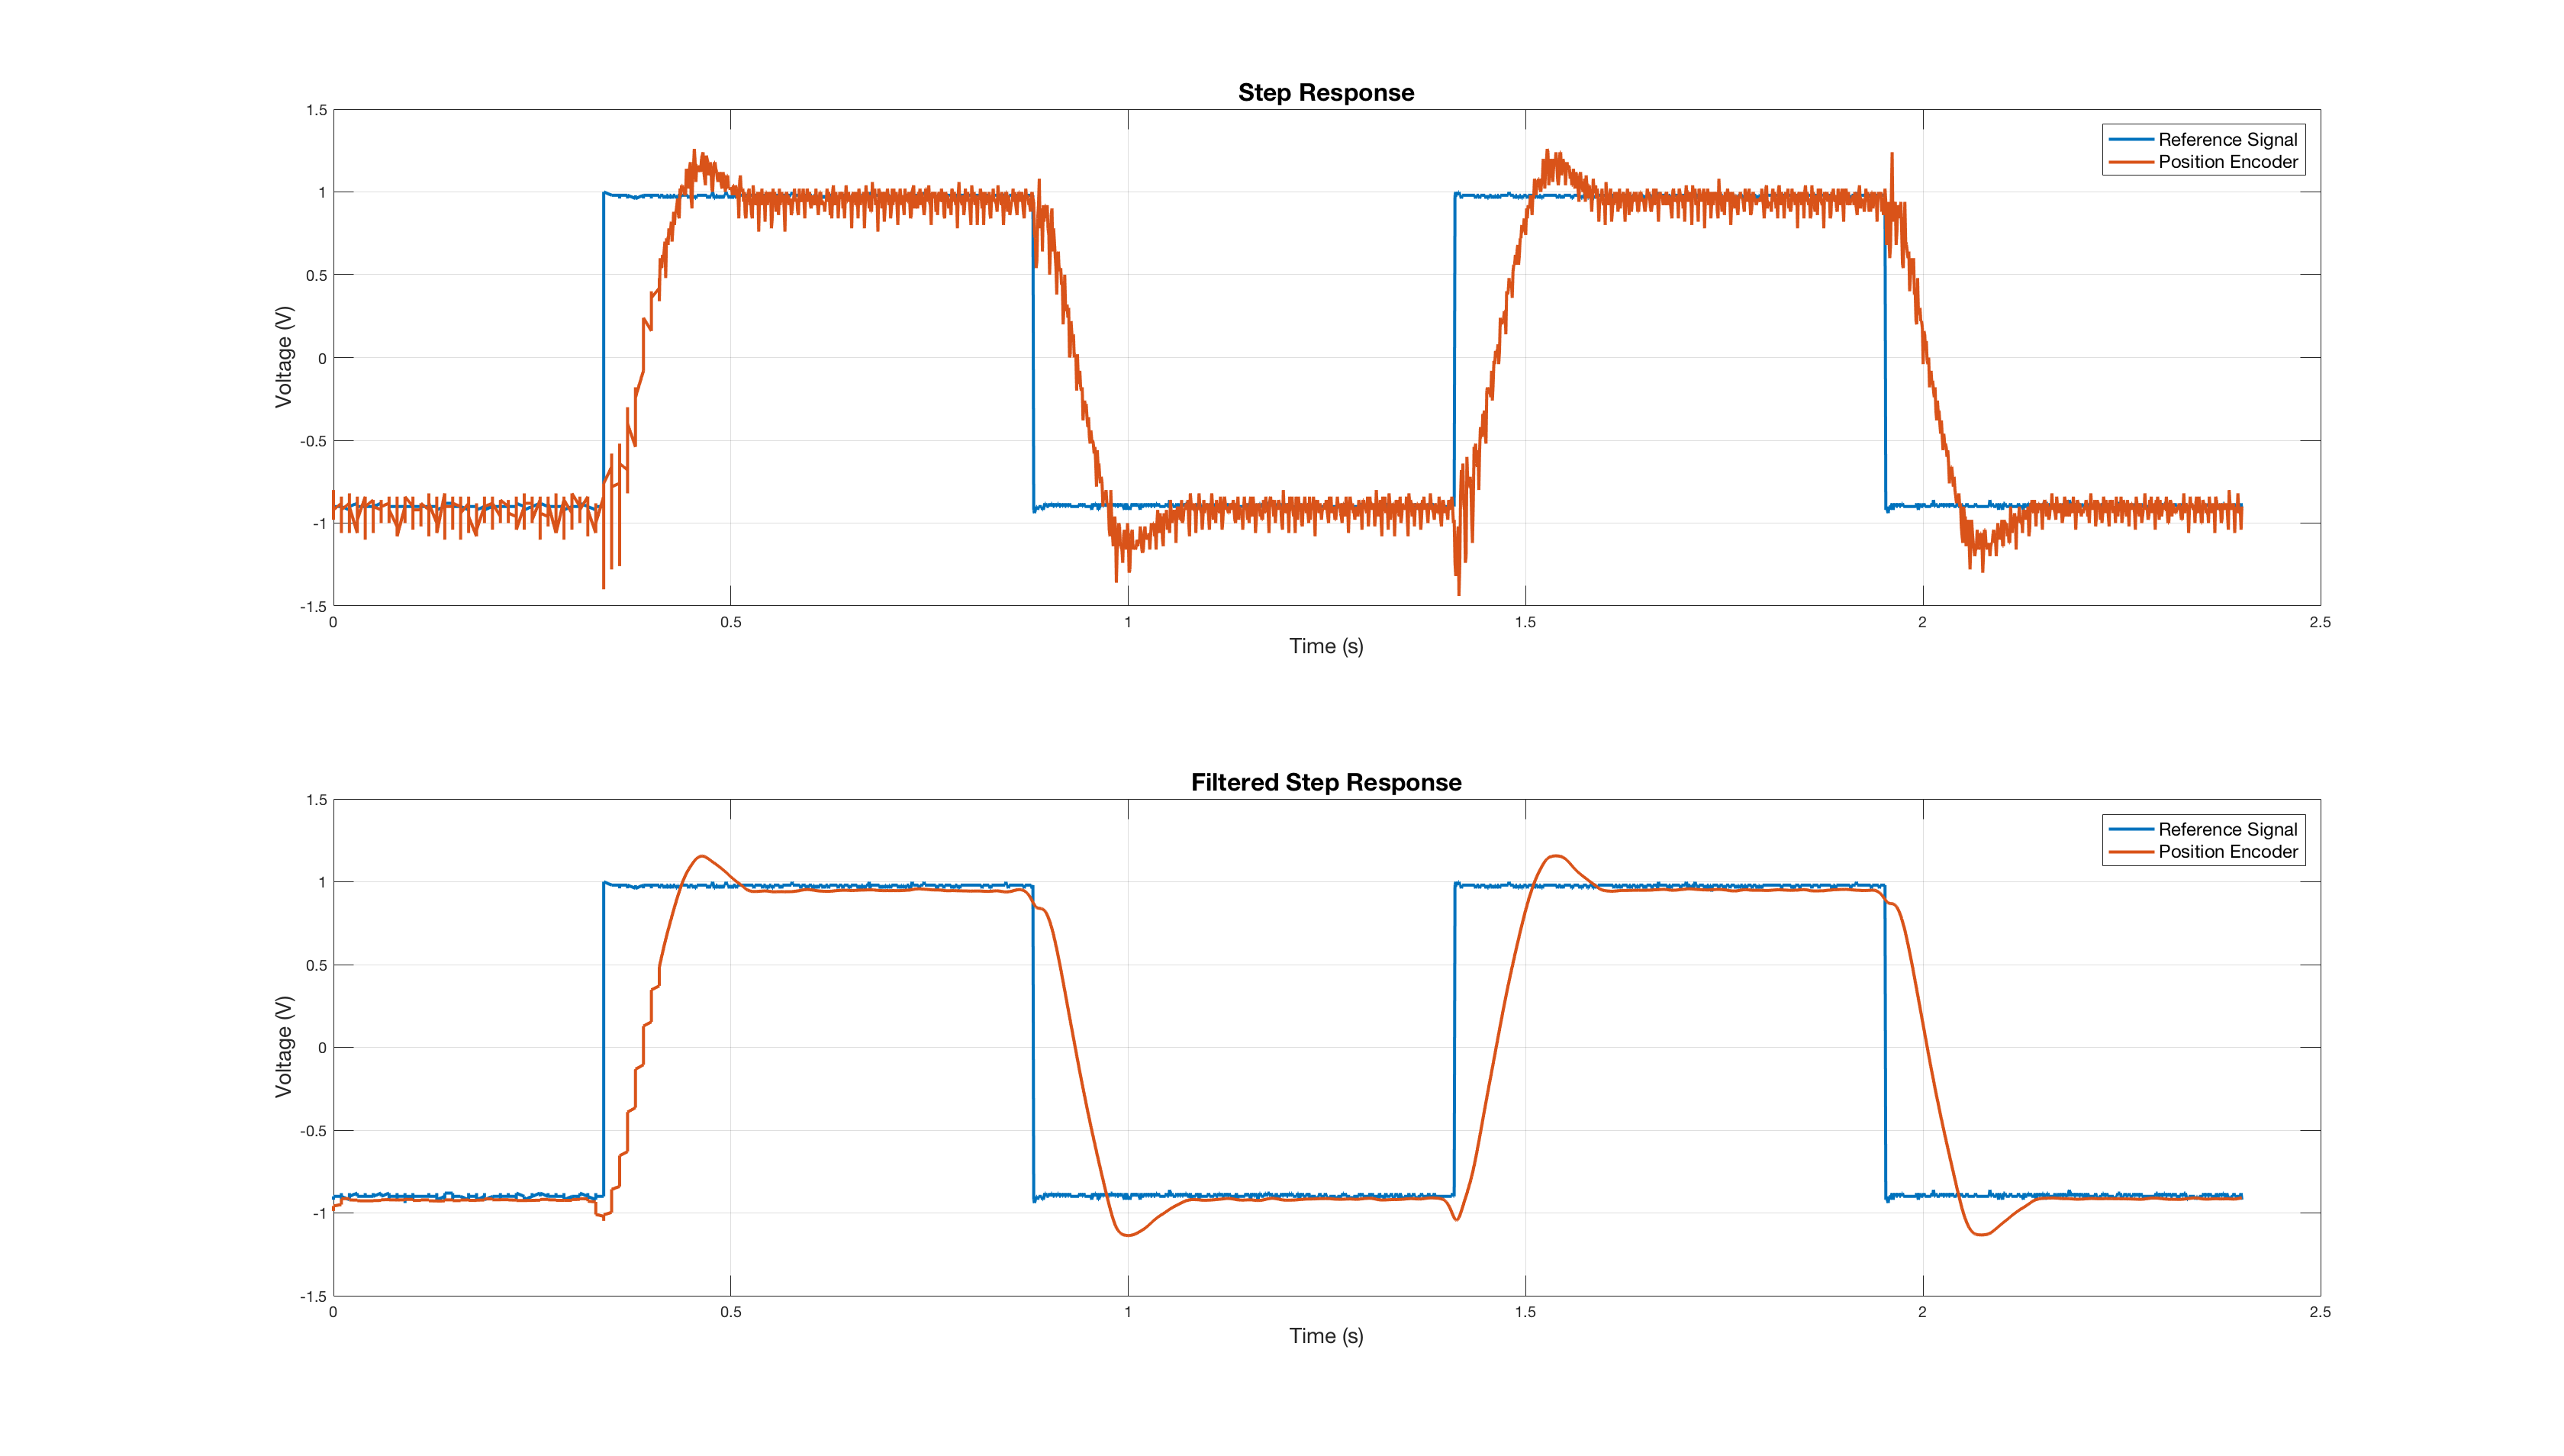
\includegraphics[width=1.1\textheight]{img/results/step.png}
    \caption{Resposta do sistema à entrada degrau unitário. O sinal de referência foi gerado por um gerador de sinais, de amplitude $1V$ pico a pico e $1Hz$. O sinal de posição do carro foi lido da saída PWM do sistema Arduino. Estão representados tanto o sinal original lido no osciloscópio, como um sinal filtrado para remover ruídos de alta frequência.}
    \label{fig::step_response}
\end{sidewaysfigure}

\begin{sidewaysfigure}
	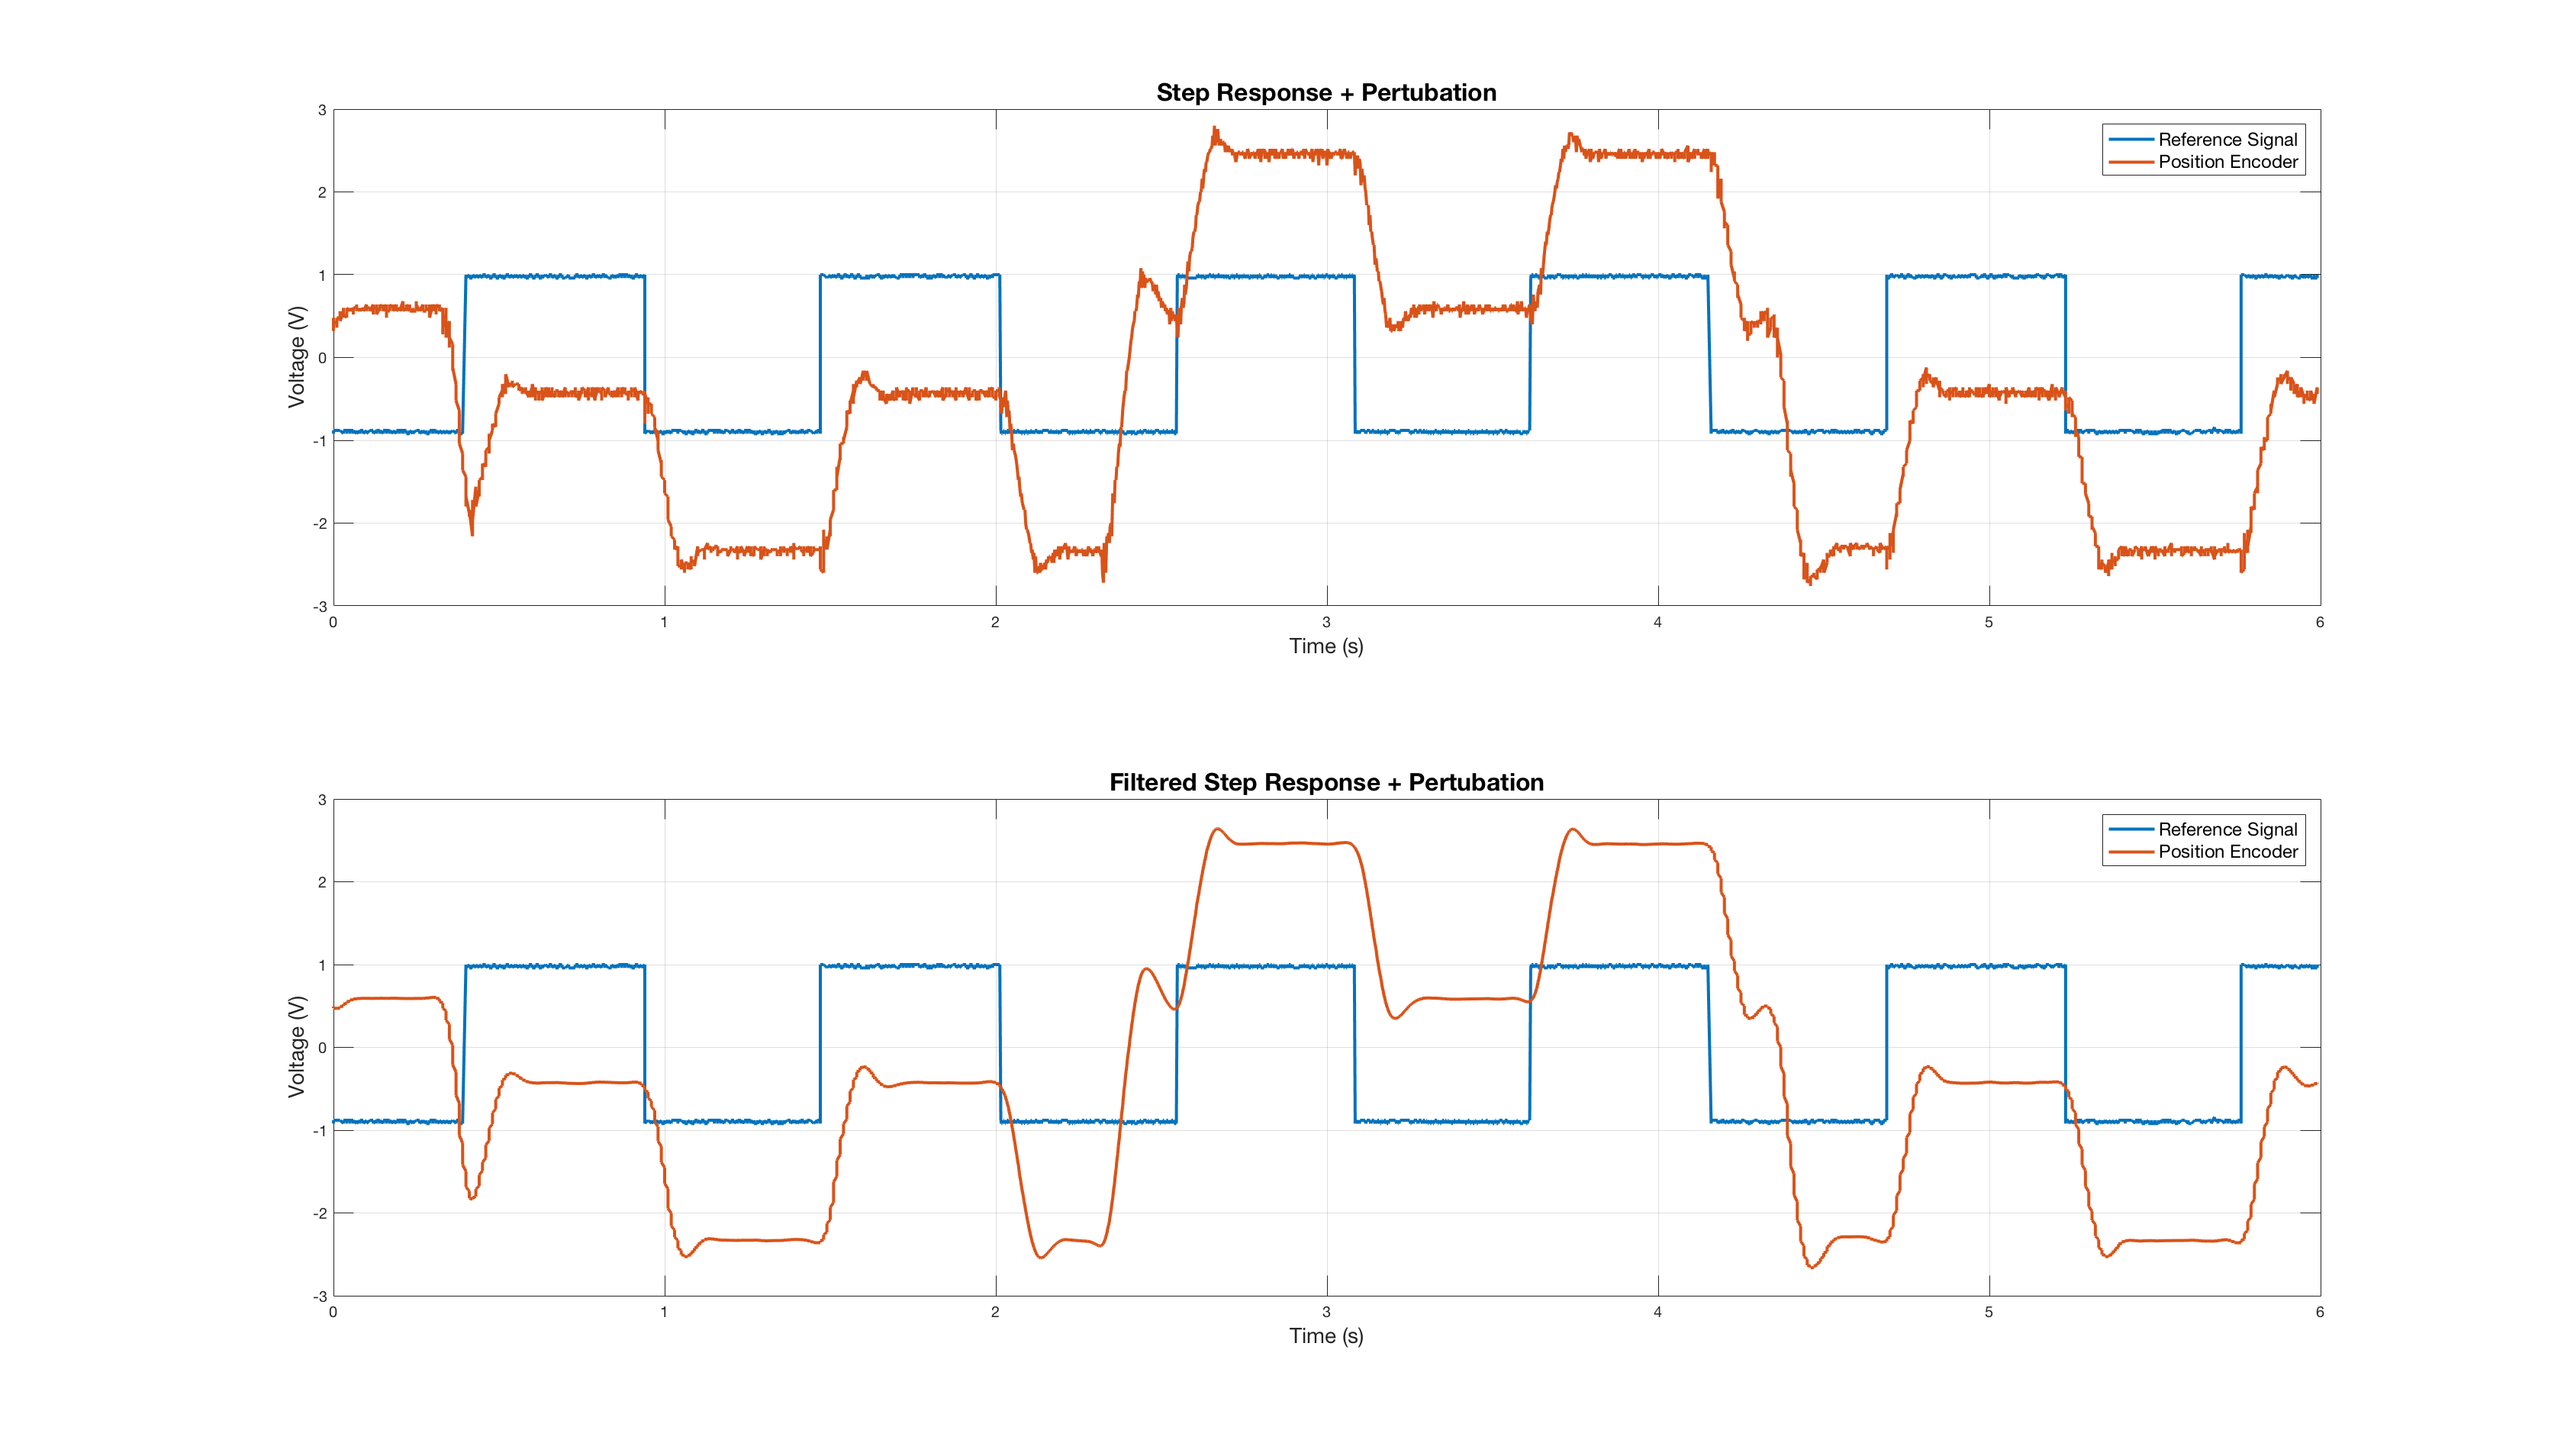
\includegraphics[width=1.1\textheight]{img/results/step_noise.png}
    \caption{Resposta do sistema à entrada degrau unitário com pertubação de $0.25 Hz$ e $2V$ pico a pico. Tanto o sinal de referência, como o sinal de perturbação foram gerados por gerador de sinais. O sinal de posição do carro foi lido da saída PWM do sistema Arduino. Estão representados tanto o sinal original lido no osciloscópio, como um sinal filtrado para remover ruídos de alta frequência.}
    \label{fig::step_noise_response}
\end{sidewaysfigure}

\begin{sidewaysfigure}
	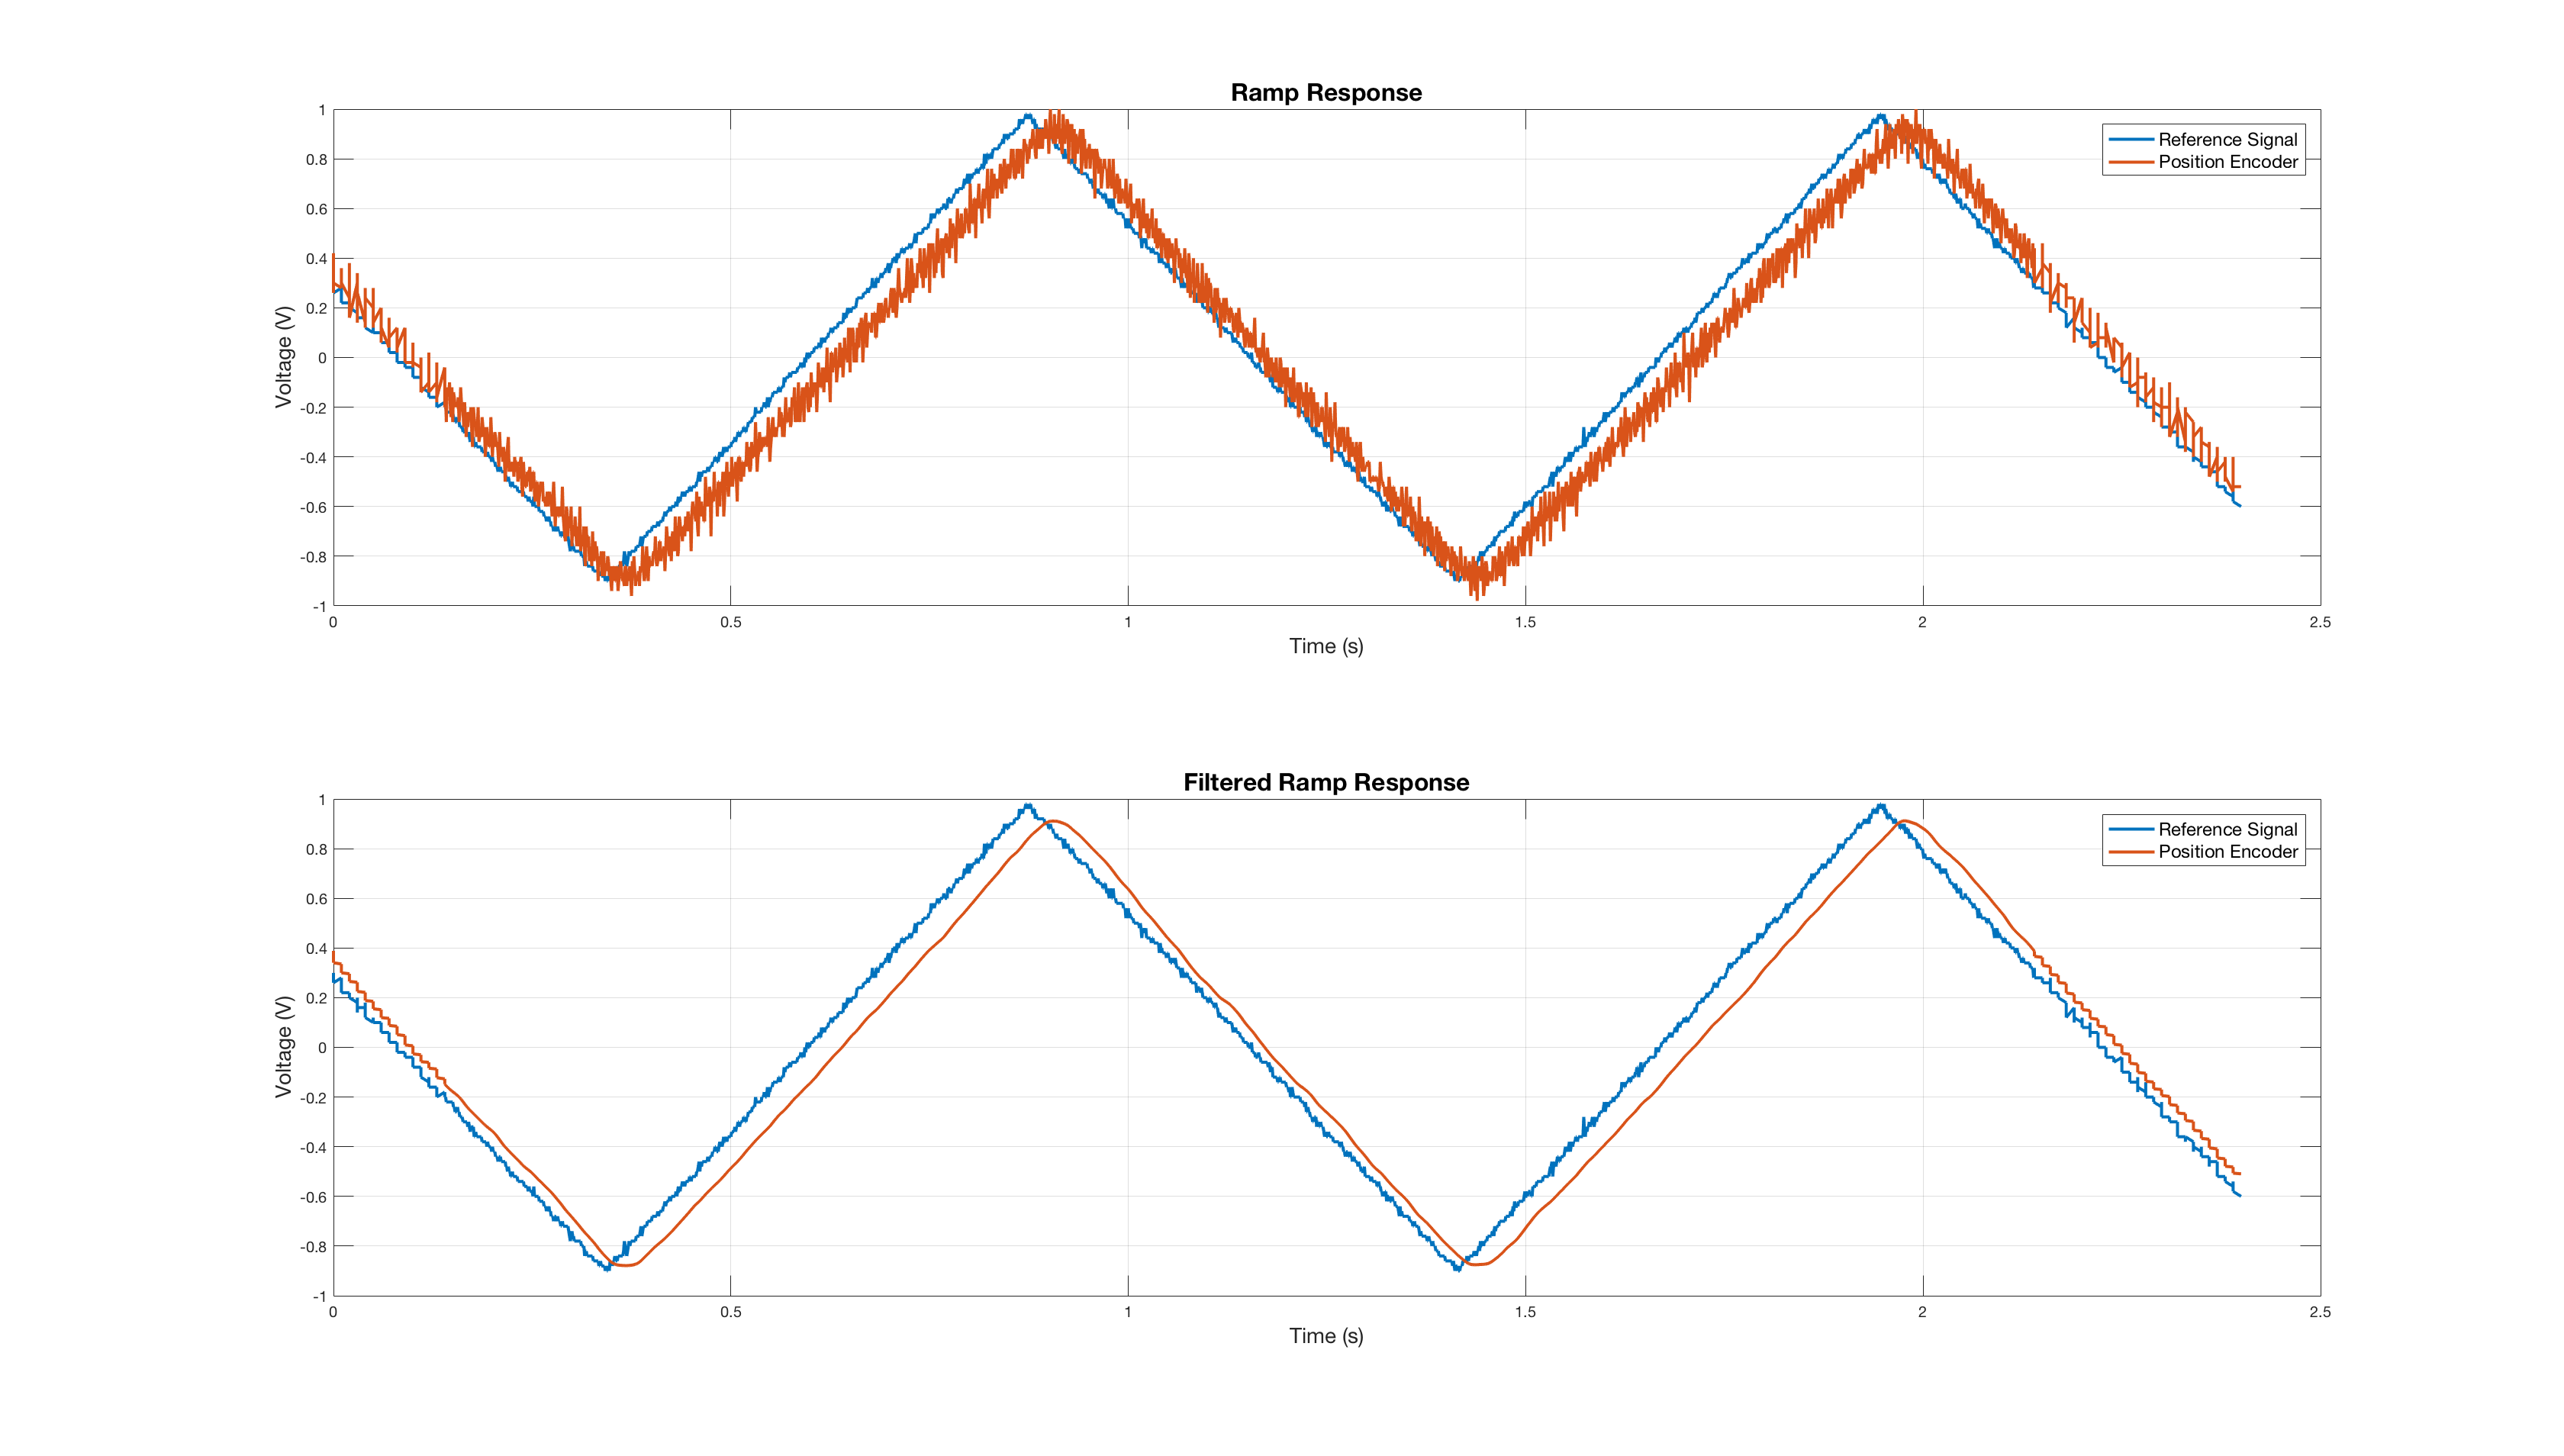
\includegraphics[width=1.1\textheight]{img/results/ramp.png}
    \label{fig::ramp_response}
    \caption{Resposta do sistema à entrada rampa unitária. O sinal de referência foi gerado por um gerador de sinais, de amplitude $1V$ pico a pico e $1Hz$. O sinal de posição do carro foi lido da saída PWM do sistema Arduino. Estão representados tanto o sinal original lido no osciloscópio, como um sinal filtrado para remover ruídos de alta frequência.}
\end{sidewaysfigure}

\begin{sidewaysfigure}
	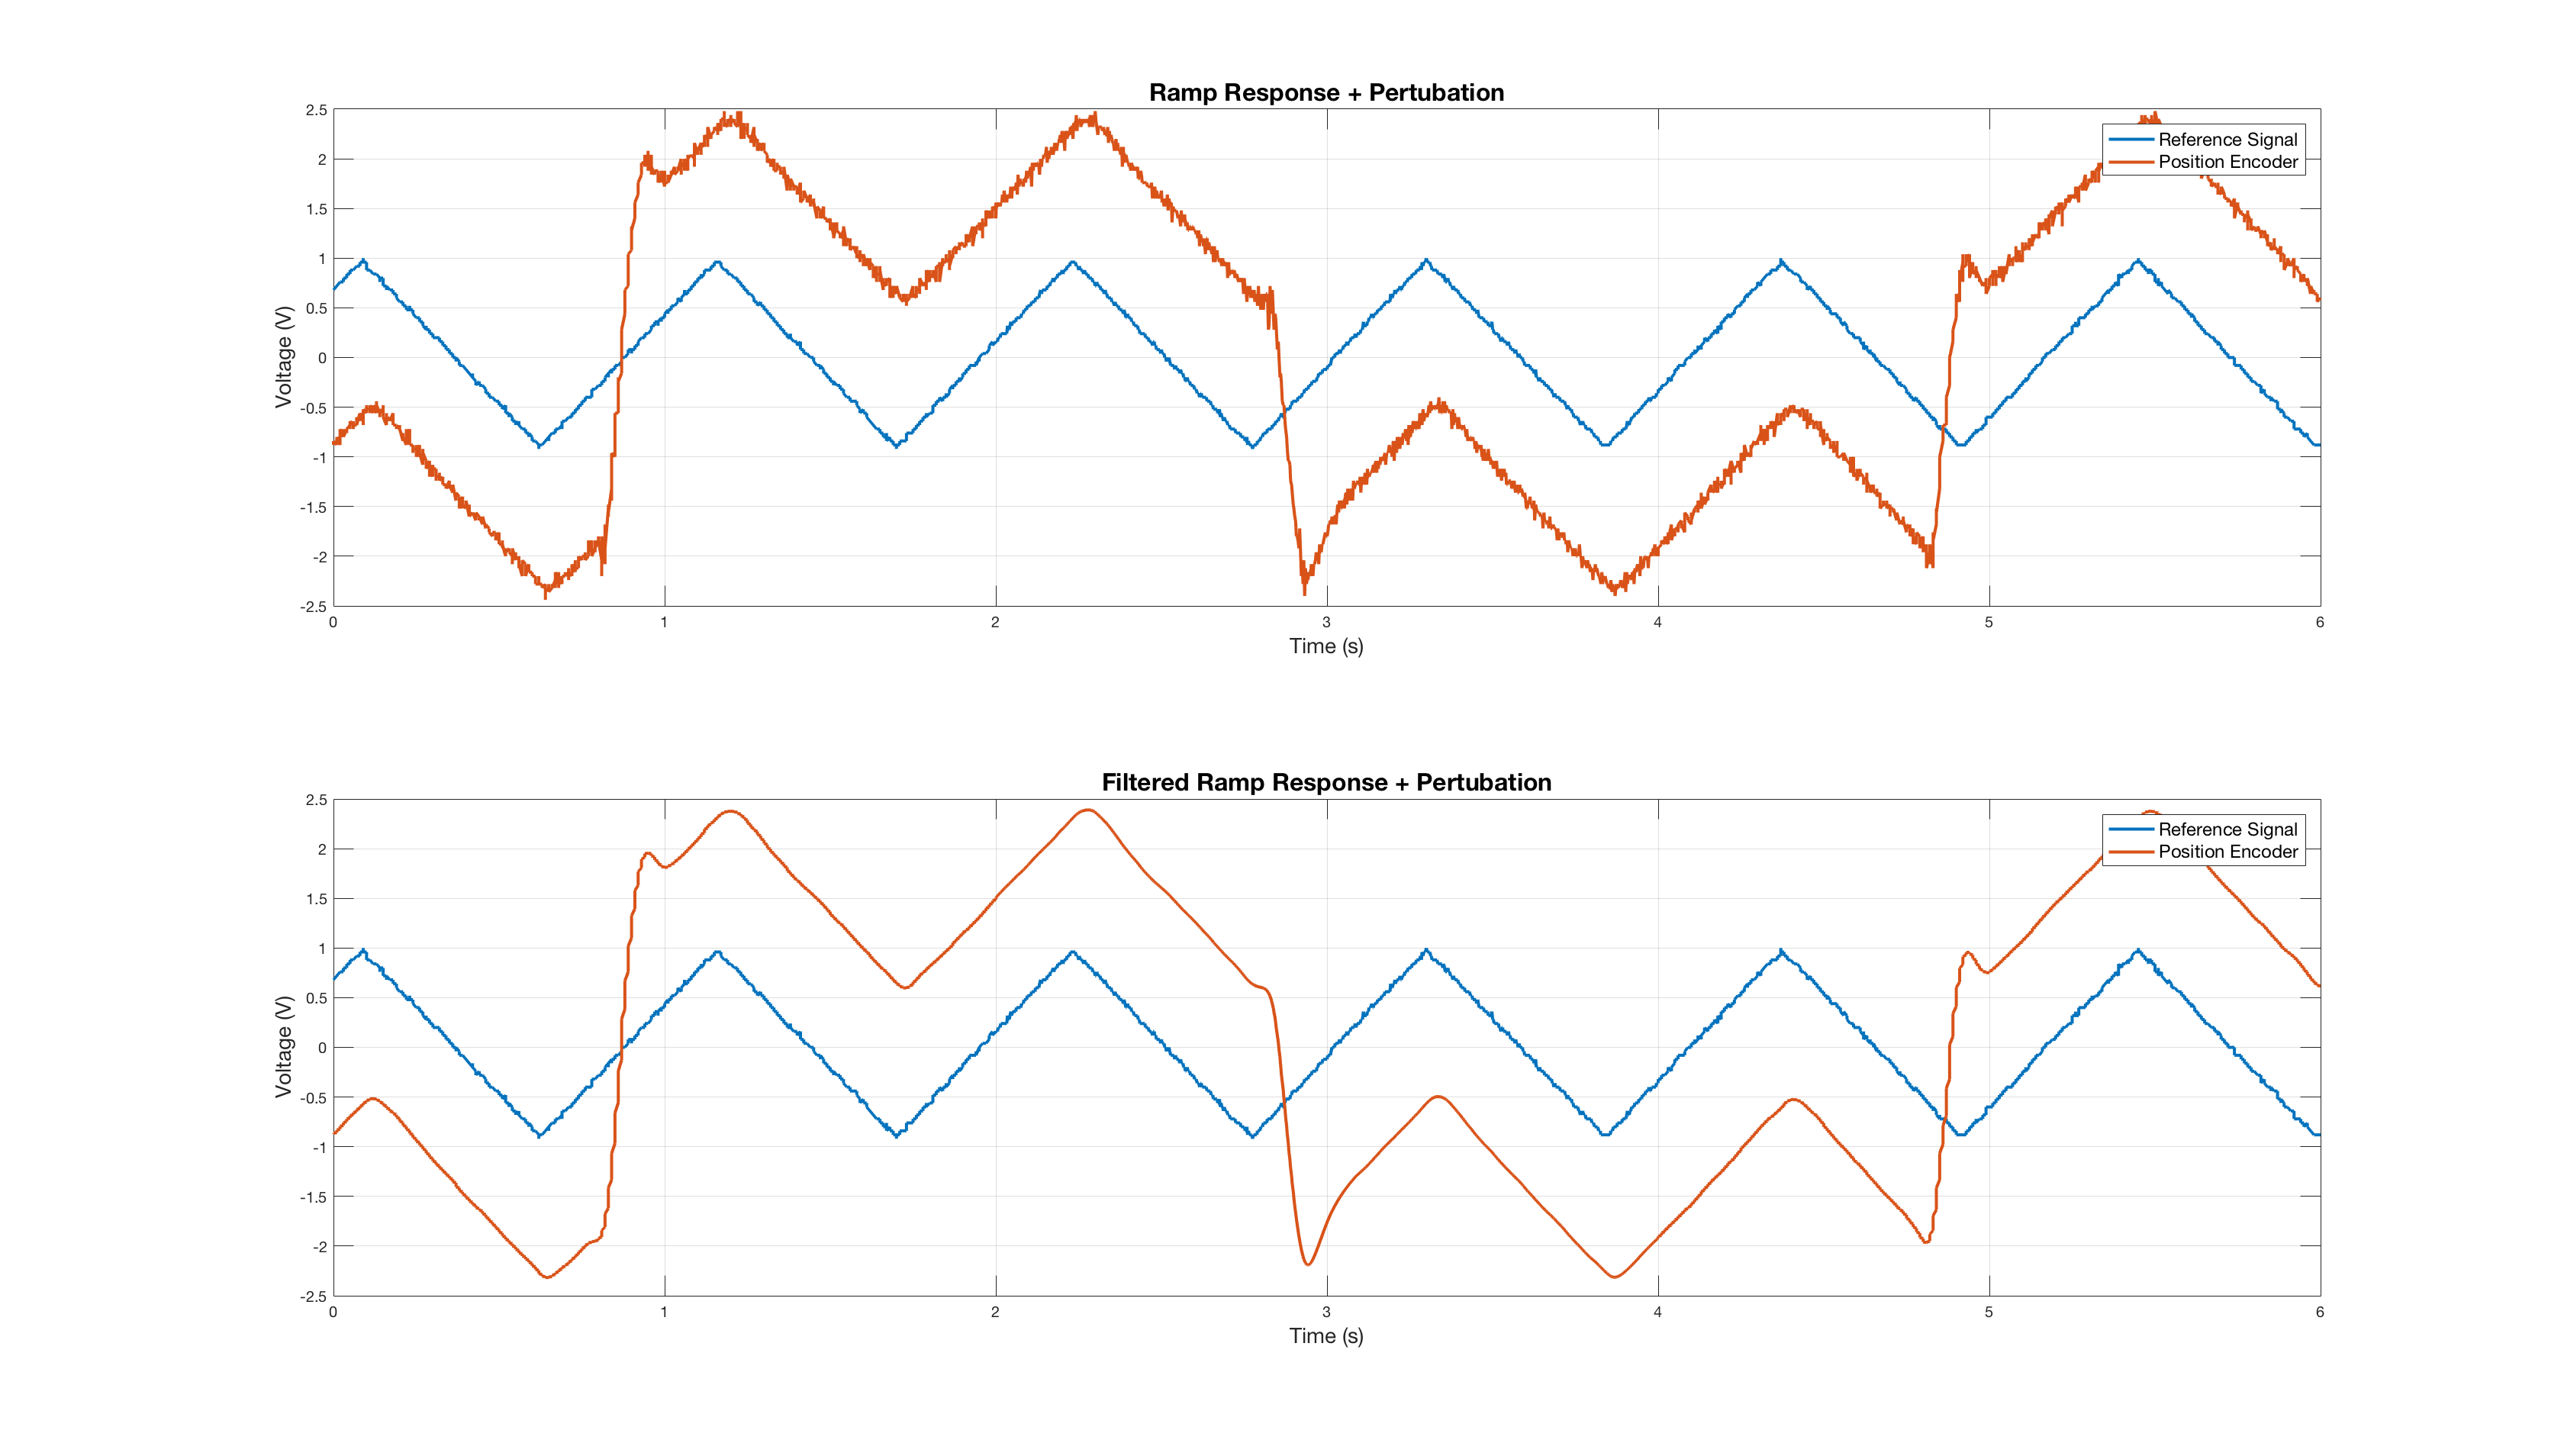
\includegraphics[width=1.1\textheight]{img/results/ramp_noise.png}
    \caption{Resposta do sistema à entrada rampa unitária com pertubação de onda quadrada de $0.25 Hz$ e $2V$ pico a pico. Tanto o sinal de referência, como o sinal de perturbação foram gerados por gerador de sinais. Estão representados tanto o sinal original lido no osciloscópio, como um sinal filtrado para remover ruídos de alta frequência.}
    \label{fig::ramp_noise_response}
\end{sidewaysfigure}


O experimento foi realizado em conformidade às instruções \cite{CDIN:Roteiro1} resumidas na seção \ref{sec::materiais_metodos}. Os dados foram adquiridos por meio dos canais de osciloscópios digitais e exportados para ambiente MATLAB.

A resposta do sistema ao degrau unitário encontra-se expresso na figura \ref{fig::step_response}. Adicionando-se a perturbação em forma de onda quadrada, o sistema comporta-se conforme a figura \ref{fig::step_noise_response}. As curvas observadas para o sinal de referência rampa unitária estão expressas na figura \ref{fig::ramp_response}. Ao adicionar-se a perturbação, o sistema assume o comportamento da figura \ref{fig::ramp_noise_response}.

Faz-se importante mencionar que o período de amostragem não mostrou-se constante nos dados adquiridos. Contudo, para efeitos de análise deste relatório, utilizamos a moda da distribuição: $1ms$.